%BAB_3 LAPORAN KP

\chapter{PERANCANGAN SISTEM}
Pada bab ini akan disajikan mekanisme perancangan alat, baik perangkat keras ataupun perangkat lunak untuk mewujudkan sebuah robot lengan. Tahapan perancangan dimulai dari perancangan diagram blok sistem, perancangan perangkat keras, perancangan perangat lunak, perancangan kinematika balik, dan integrasi keseluruhan program. 
\section{ Diagram Blok Sistem }
Secara garis besar, pada tahapan implementasi dari kinematika pada \textit{arm manipulator robot} SCARA ini menggunakan output atau penggerak berupa motor DC dengan \textit{feedback} posisi berupa potensiometer dan pada bagian  input yang berasal dari Processing IDE yang mengirimkan sebuah koordinat yang digunakan untuk menentukan pergerakan robot berdasarkan fungsi \textit{inverse kinematic}. Sistem kerja \textit{arm manipulator robot} SCARA ditunjukan pada  Gambar 3.1.
\begin{figure}[H]
	\centering
	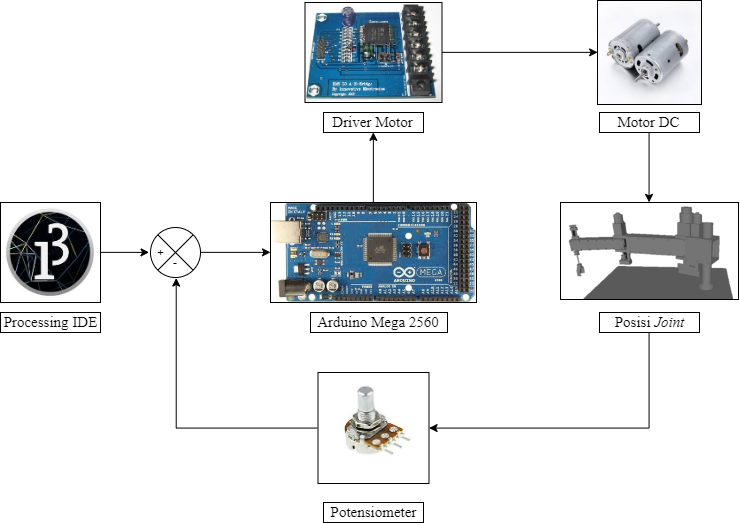
\includegraphics[width=12cm]{gambar/Rangkaian_Diagram.png}
	\caption{Diagram Blok Sistem}
\end{figure}
Pada blok diagram yang disajikan pada Gambar 3.1 sistem terdiri dari bagian – bagian yang meliputi bagian masukan, bagian kendali, bagian keluaran, dan bagian penampil. Pada bagian masukan menggunakan GUI yang dirancang pada Processing IDE yang digunakan sebagai \textit{forward kinematic} serta \textit{inverse kinematic} dimana robot akan bergerak menyesuaikan dengan posisi atau sudut yang diinputkan melauli Processing IDE. 
Pada bagian kontrol menggunakan Arduino Mega 2560 sebagai mikrokontroler yang mengendalikan seluruh operasi dari robot. \textit{Power supply} Arduino sebesar 5 volt DC didapatkan dari regulator tegangan yang menurunkan tegangan dari 12 volt DC ke 5 volt DC. 

Pada bagian keluaran, pin pulse with modulation (PWM) pada Arduino Mega 2560 dihubungkan dengan driver motor yang digunakan untuk mengontrol arah pergerakan dari motor DC serta kecepatan pergerakan dari motor DC. Pergerakan arah putaran motor DC bergantung pada \textit{feedback} posisi setiap sendi yang diberikan oleh potensiometer. Tiga buah pin digital ardunio dihubungkan rangkaian \textit{switch} yang menggunakan IC TIP31 yang berfungsi sebagai kontrol dari \textit{End-Effector} dari robot SCARA.

Pada bagian penampil merupakan bentuk dari rancangan GUI yang dirancang dalam Processing IDE melalui sebuah bentuk pemrograman. Dalam tampilan GUI nya, terdapat beberapa \textit{tools} yang dapat untuk mengatur pergerakan robot SCARA. Pada GUI juga dapat menampilkan nilai dari sudut, dan posisi pada kondisi langsung dari pergerakan robot SCARA.
\section{ Perancangan Perangkat Keras }
Perancangan perangkat keras pada \textit{arm manipulator robot} SCARA terdiri dari dua bagian yaitu bagian mekanik dan elektronis. Bagian  mekanik merupakan bagian \textit{hardware} yang meliputi desain, bahan dan bentuk dari arm manipulator robot SCARA dan bagian elektronis merupakan bagian \textit{hardware} yang meliputi sistem – sistem yang berkaitan dengan rangkaian pada I SCARA seperti rangkain pada desain \textit{board} serta komponen – komponen elektronis.
\subsection{ Sistem Mekanik }
Sistem mekanika dari robot lengan bergantung dari konfigurasi robot lengan. Konfigurasi robot lengan terbagi menjadi enam, yaitu konfigurasi \textit{Articulated}, konfigurasi SCARA, konfigurasi \textit{Spherical}, konfigurasi \textit{Cylindrical}, dan konfigurasi \textit{Cartesian}. Pada tugas ini, konfigurasi robot lengan yang digunakan adalah konfigurasi SCARA, dengan dua joint revolute dan satu \textit{end-effector}. Sistem mekanik dari lengan robot tiga DOF sangat berpengaruh dan mendominasi sistem karena bentuk dan pergerakan dari mekanik akan mempengaruhi elektronis, serta program. Sistem mekanik yang baik sangat mendukung dari pergerakan robot, oleh karena itu perancangan mekanik haruslah proporsional dari panjang setiap lengan, lebar serta tinggi robot. Pada Gambar 3.2 disajikan \textit{free body} dari robot SCARA.
\begin{figure}[H]
	\centering
	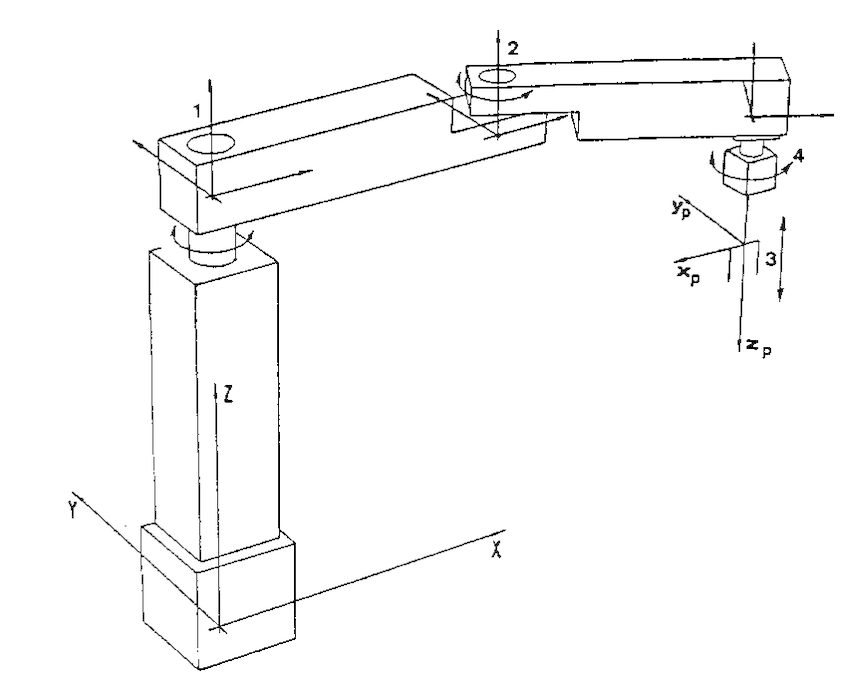
\includegraphics[width=7cm]{gambar/scaraa.png}
	\caption{\textit{Free Body} Robot Scara}
\end{figure}
 Struktur \textit{joint} dari robot lengan dengan DOF berjumlah tiga adalah \textit{shoulder}, \textit{elbow}, dan \textit{end-effector}. \textit{Joint} dikendalikan dengan motor DC yang didalamnya terdapat rangakain \textit{gear} agar motor DC dapat bekerja seperti motor servo.  Sedangkan pada \textit{end-effoctor} tidak digunakan motor DC melainkan menggunakan \textit{valve relay pneumatic} dengan sistem kerja translasi yang dikombinasikan dengan desain mekanik sehingga dapat membuat dua buah gerakan, yaitu naik turun dan buka tutup pada \textit{gripper}. Pada \textit{arm manipulator robot} SCARA memiliki spesifikasi yang dijelaskan pada tabel 3.1.
 
\begin{table}[H]
	\centering
	\caption{Spesifikasi Robot SCARA}
	\resizebox{6cm}{!}{%
		\begin{tabular}{|l|l|}
			\hline
			Main arm length      & 360 mm$$\hspace{2cm} 		\\ \hline
			Fore arm length      & 290 mm$$  				\\ \hline
			Shoulder movement    & 180 °$$  		\\ \hline
			Elbow movement       & 200 °$$   		\\ \hline
			Wrist rotation       & 360 °$$ 		\\ \hline
			Up \& down movement  & 150 mm$$   				\\ \hline
			Maximum tip velocity & 3.0 kg$$  				\\ \hline
			
			\end{tabular}%
		}
		\end{table}

 
Perancangan robot serpent-2 ini diawali dengan menentukan metode yang tepat untuk mendesain dan membangun sistem secara keseluruhan meliputi perancangan elektronis,pemrograman pada Arduino Mega 2560, implementasi kinematika robot pada robot serpent-2, serta perancangan antarmuka pada \emph {processing ide}.Metode perancangan sistem meliputi diagram blok, flowchart cara kerja sistem, prinsip kerja dan perancangan tiap segmen-segmen yang dibutuhkan.
	
	\subsection{Diagram Blok Perancangan Sistem}
	Pada dasarnya, perancangan sistem untuk robot serphent-2 secara sederhana dapat dibagi menjadi tiga bagian. Ketiga perancangan ini merupakan hal yang sangat penting dan saling berkaitan.Perancangan robot serphent=2 jika digambarkan dalam diagram blok sistem dapat digambarkan seperti yang ditunjukkan dalam gambar 3.1
	\begin{figure}[H]
		\centering
		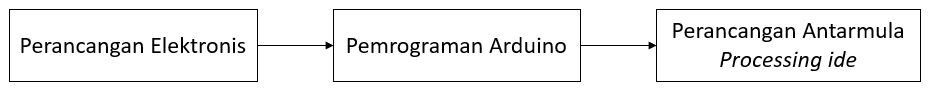
\includegraphics[width=\linewidth]{gambar/diagram_blok.jpg}
		\caption{Diagram metode perancangan sistem.}
	\end{figure}

\subsection{Flowchart Cara Kerja Sistem}
Kerja sistem, merupakan bagaimana robot serphent-2 melakukan tugasnya sesuai perintah yang dimasukkan dan kemudian dilaksanakan oleh aktuator.Robot serphent-2 memiliki kerja sistem yang tergolong ringkas yang mana didominasi oleh sistem maju tetapi juga memiliki sistem balik.  Kerja sistem dari robor serphent 2 jika dirancang dalam bentuk flowchat dapat ditunjukkan seperti dalam gambar 3.2

\begin{figure}[H]
	\centering
	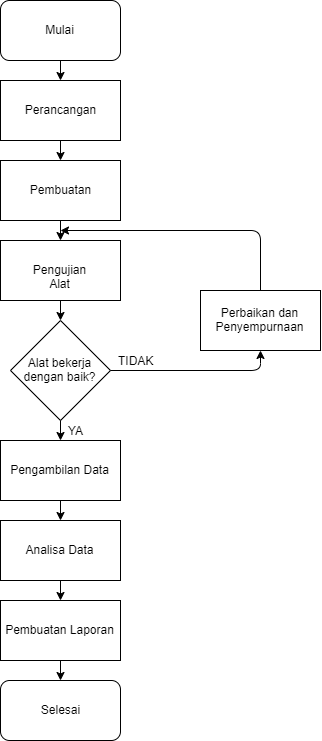
\includegraphics[width=8cm	]{gambar/flowchart.png}
	\caption{Flowchat cara kerja sistem.}
\end{figure}
	
	\subsection{Perancangan Elektronis}
	Perancangan elektronis merupakan perancangan dasar pada pembuatan suatu sistem. Suatu sistem dapat bekerja secara maksimal karena terdiri dari komponen-komponen yang memiliki fungsi masing-masing. Komponen-komponen ini, disatukan kedalam sebuah \textit{Shield} \textit{Printed Circuit Board} (PCB). 
	
	\begin{enumerate}
		\item Pengendali motor DC yang digunakan adalah modul EMS 30A H-Bridge sebanyak tiga buah yang masing-masing untuk menggerakkan \textit{Shoulder, Elbow} dan perputaran \textit{Wrist}. Secara garis besar, fungsi modul pengendali motor ini adalah untuk mengendalikan arah dan kecepatan putaran motor DC sesuai instruksi kendali dari Arduino Mega 2560 pengguna.Modul akan menerima nilai yanf dikirimkan oleh Arduino Mega 2560 dan kemudian menggerakan motor servo yang sudah terhubung dengan \textit{shoulder, Elbow} dan perputaran dari \textit{Wirst}.
		
		\begin{figure}[H]
			\centering
			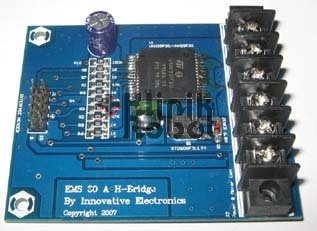
\includegraphics[width=5cm	]{gambar/driver_motor.jpg}
			\caption{Pengendali Motor DC EMS 30A H-Bridge}
		\end{figure}
		
		\item Potensiometer yang digunakan adalah jenis potensiometer \textit{rotary}. Potensiometer ini sebagai sensor posisi motor servo. Potensiometer terpasang pada setiap bagian motor servo sesuai dengan perputarannya dan akan memberikan keluaran berupa level tegangan yang berubah-ubah sesuai dengan posisi motor servo saat itu. Level tegangan tersebut kemudian dikirimkan kepada Arduino Mega 2560 sebagai sensor \textit{feedback} yang nantinya akan diproses untuk menyempurnakan posisi sesuai yang ditentukan.
		\begin{figure}[H]
			\centering
		%	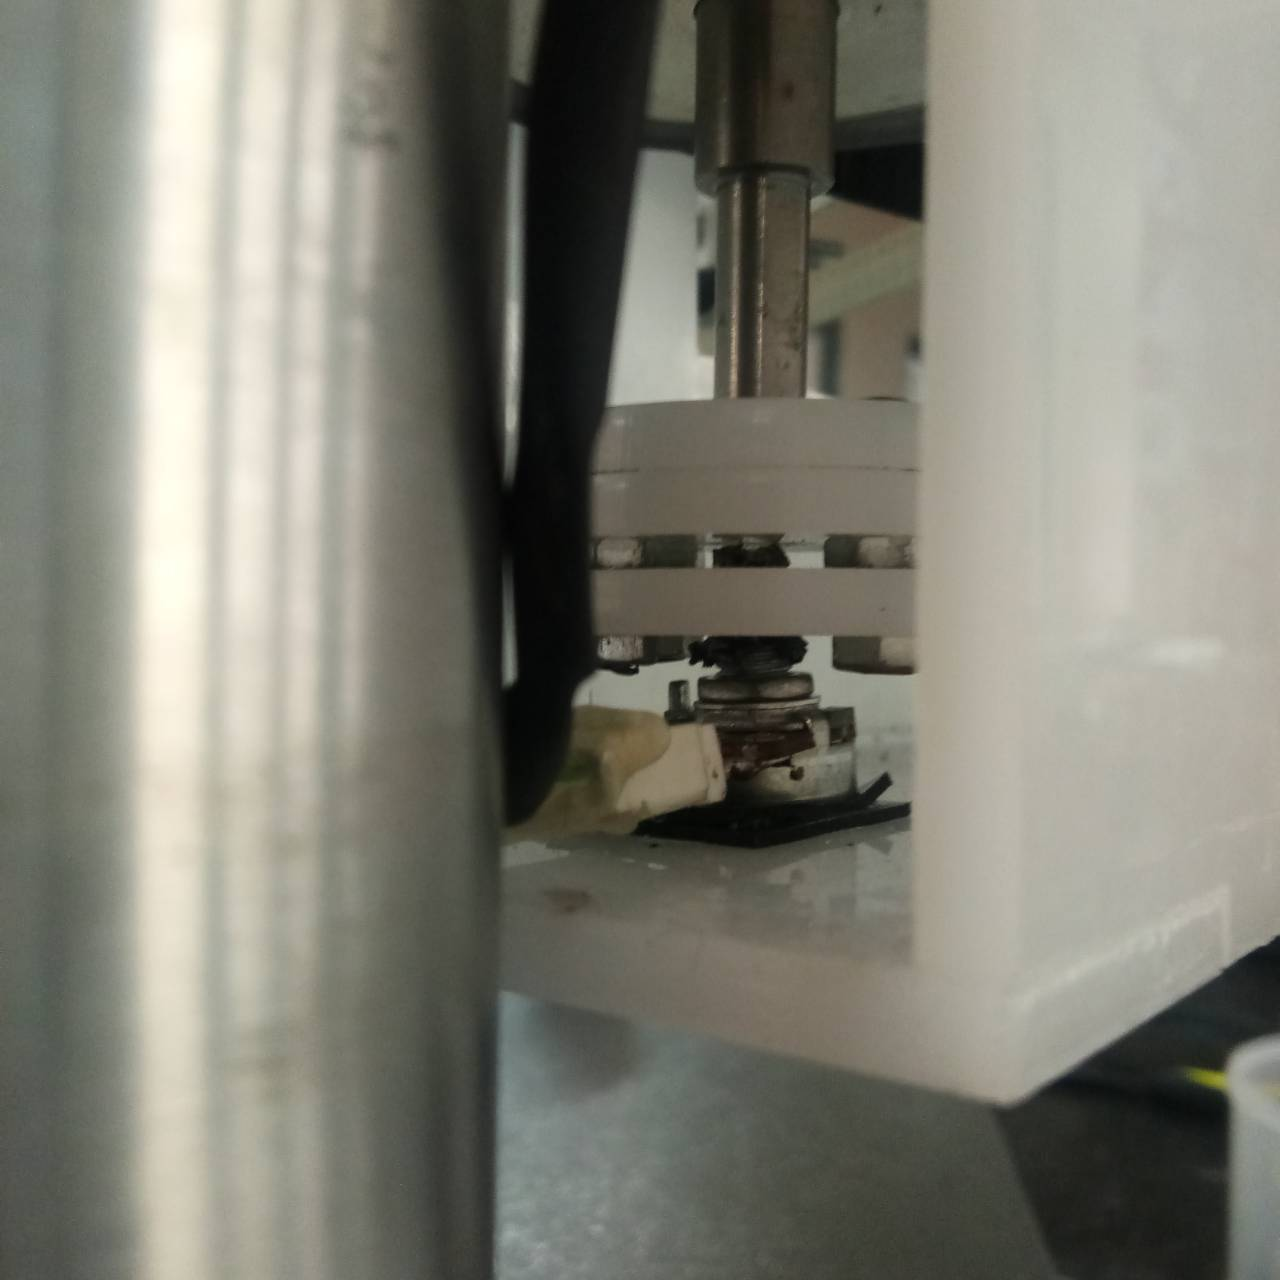
\includegraphics[width=5cm	]{potensio.jpg}
			\caption{Mekanisme pemasangan potensiometer pada motor}
		\end{figure}
		
		\item Pengaturan pergerakan vertikal dari \textit{wirst} pada robot serphent-2 menggunakan sistem pneumatik silinder. Pada bagian buka tutup \textit{wirst} menggunakan masukan udara biasa untuk menutupnya dan membuang udara unutk membukanya. Udara tersebut didapat dari kompresor yang terhubung melalui selang dan dikontrol melalui sebuah relay yang bekerja pada tegangan 24v.
		
		\begin{figure}[H]
			\centering
		%	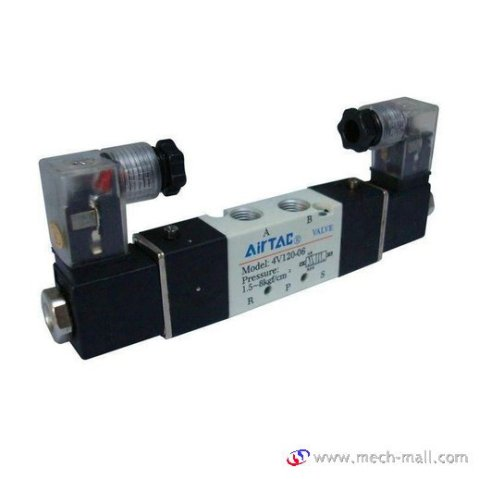
\includegraphics[width=5cm	]{relay.jpg}
			\caption{Relay pneumatik}
		\end{figure}
		\begin{figure}[H]
			\centering
		%	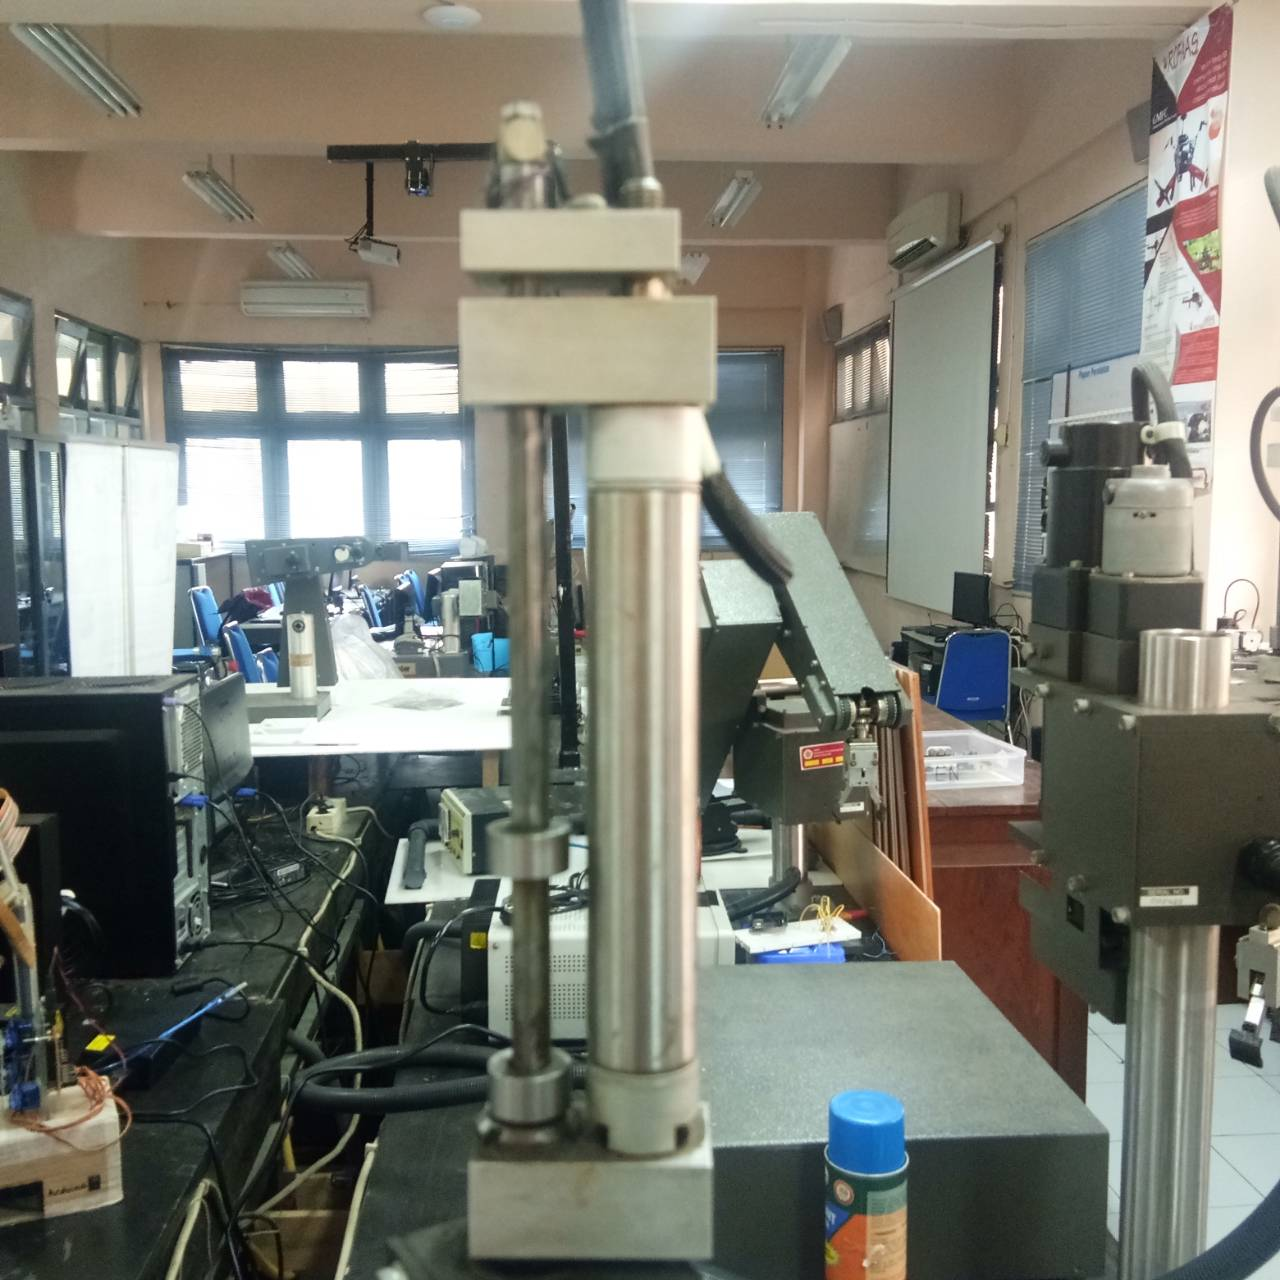
\includegraphics[width=5cm	]{relay2.jpg}
			\caption{Pneumatik Silinder}
		\end{figure}
		
		\item Relay yang bekerja pada tegangan 24v, pada Arduino Mega 2560 dikontrol melalui sinyal digital dengan bantuan rangkaian yang menggunakan TIP31A yang berfungsi untuk memutus atau membuka tegangan 24v. 
		\begin{figure}[H]
			\centering
		%	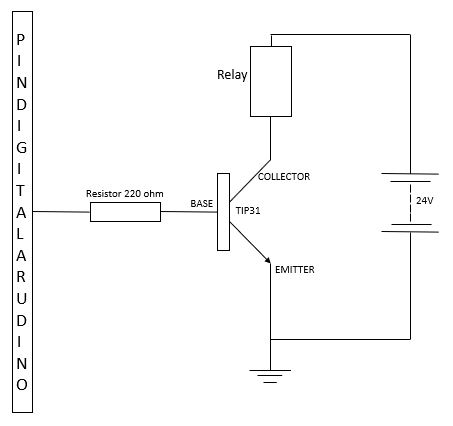
\includegraphics[width=5cm	]{relay3.jpg}
			\caption{Rangkaian skematik TIP31 sebagai \textit{switch}}
		\end{figure}
		
		\item Semua komponen-komponen yang dibutuhkan pada sistem kerja, disatukan ke dalam \textit{shield PCB} yang bertujuan agar meringkaskan serta memudahkan perangkaian elektronis. Rangkaian PCB dibuat melalui \textit{software} Eagle.
		\begin{figure}[H]
			\centering
		%	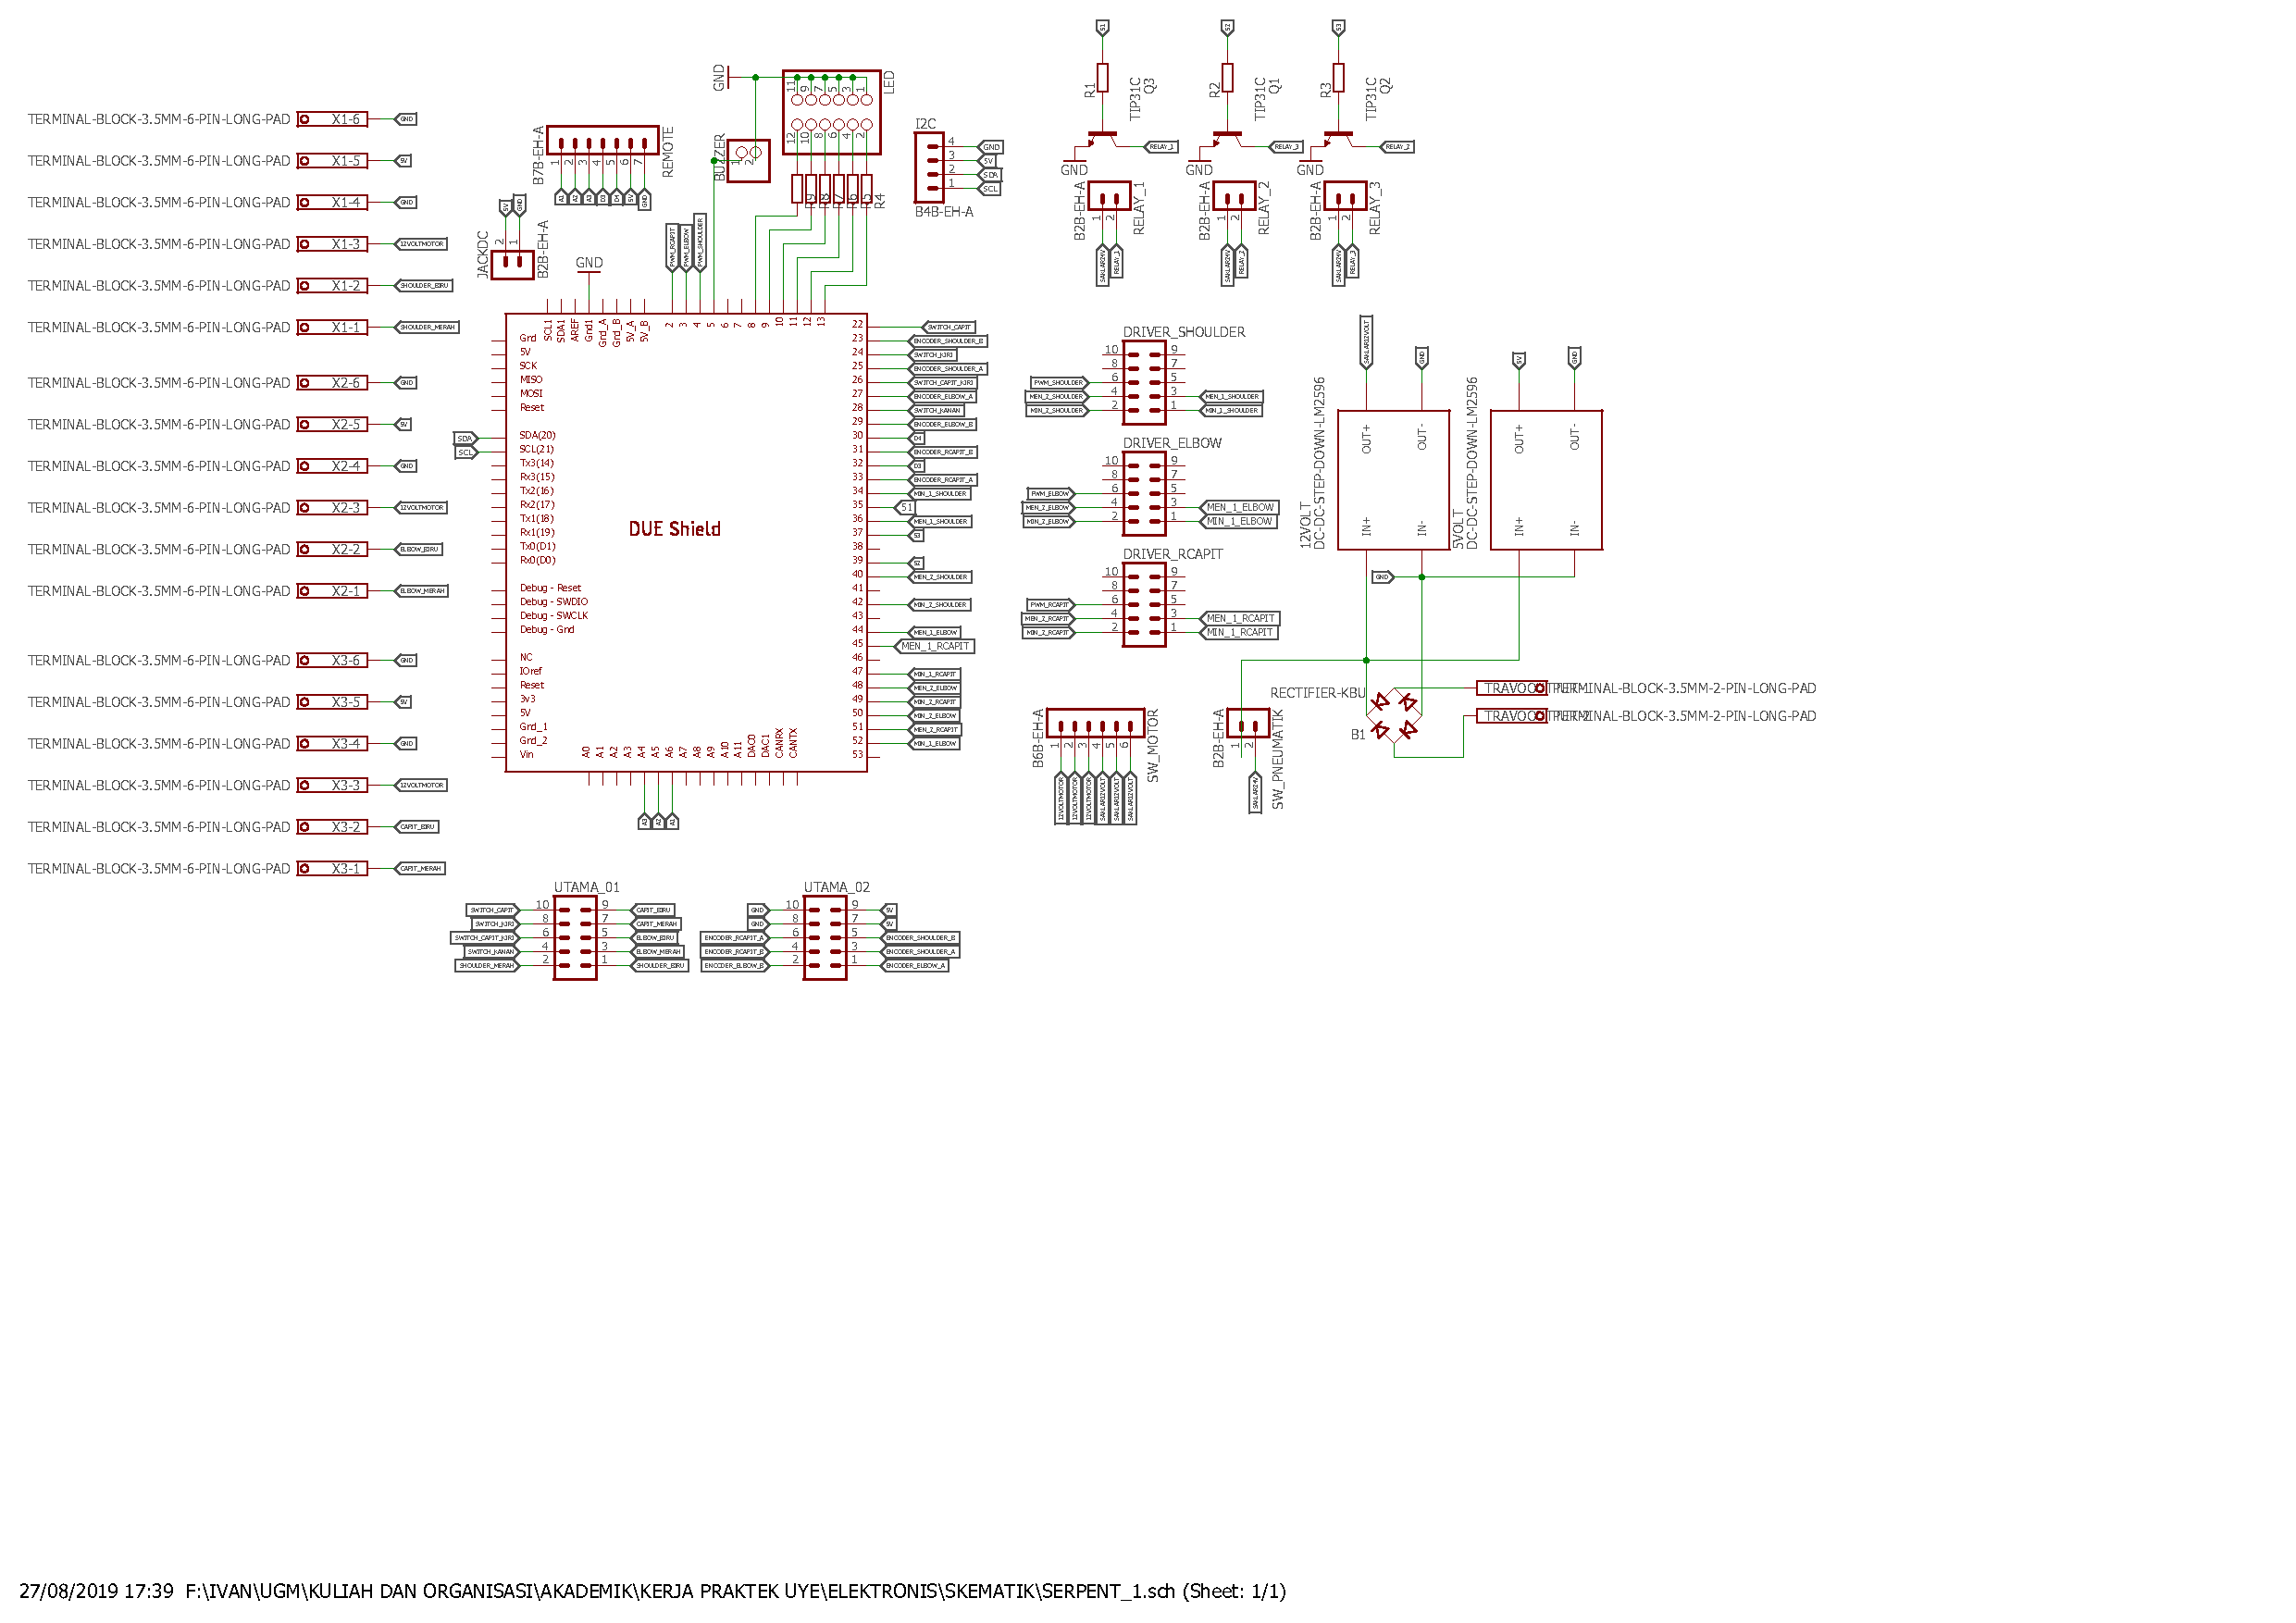
\includegraphics[width=15cm	]{skematik.pdf}
			\caption{Skematik rangkaian elektronis keseluruhan}
		\end{figure}
		
		
	\end{enumerate}



SCARA merupakan singkatan dari \emph{Selective Compliant Assembly Robot Arm}. Robot ini pertama kali dibuat oleh perusahaan USA bernama Adept pada 1984 dan diklasifikasikan sebagai robot industri. Sistem penggerak robot SCARA merupakan pergerakan langsung pada lengan tanpa bantuan sistem \emph{belt} keculai pada bagian \emph wirst, sehingga membuat mekanisme gerakannya bekerja cepat, sederhana namun tetap akurat. Robot ini banyak digunakan sebagai robot \emph {aseembly part} dengan ukuran yang kecil degan kecepatan sedang. 


Robot SCARA yang digunakan pada penelitian ini menggunakan robot SCARA dengan nama Serpent-2. Robot Serpent-2 memiliki dua \textit{horizontal joint} yaitu bagian \textit{shoulder, elbow}dan \textit{wrist} yang dikendalikan oleh motor servo. Sedangkan pada bagian \textit{vertical joint} yang berfungsi sebagai naik turun dan buka tutup dari \emph wirst, dikendalikan oleh pneumatik yang dikontrol oleh \emph {valve relay}. Sehingga, gerakan yang terdapat pada robot SCARA dapat diklasifikasikan sebagai gerakan mengambil dan menempatkan objek. 


\begin{table}[H]
	\centering
	\caption{Spesifikasi Robot Serpent-2}
	\resizebox{6cm}{!}{%
		\begin{tabular}{|l|l|}
			\hline
			Main arm length      & 360 mm$$\hspace{2cm} 		\\ \hline
			Fore arm length      & 290 mm$$  				\\ \hline
			Shoulder movement    & 180 °$$  		\\ \hline
			Elbow movement       & 200 °$$   		\\ \hline
			Wrist rotation       & 360 °$$ 		\\ \hline
			Up \& down movement  & 150 mm$$   				\\ \hline
			Maximum tip velocity & 3.0 kg$$  				\\ \hline
			
			\end{tabular}%
		}
		\end{table}
		
		Pada bagian motor servo, robot serpent-2 menggunakan tiga buah sensor \emph feedback yang berguna sebagai pemberi nilai posisi pada masing-masing motor servo. Sensor \emph feedback yang digunakan pada robot SCARA ini menggunakan potensiometer yang memberikan nilai analog dan kemudian diproses oleh Arduino Mega 2560. Nilai ini, nantinya untuk memproses gerak kinematika dari robot SCARA tersebut sesuai dengan posisi yang diinginkan.
		
		
		
		\section{Motor servo}
		Motor servo merupakan sebuah motor DC yang memiliki sistem \textit{feedback}. \textit{feedback} pada motor servo merupakan koreksi sudut motor DC terhadap sudut referensi \cite{Younkin2002}. pada robot Serpent-1 terdapat tiga buah motor DC, motor DC	 bagian wrist dan elbow merupakan motor DC yang identik.sehingga penulis hanya fokus membandingkan spesifikasi dua motor DC yaitu motor DC yang berada di bagian shoulder (\textit{main arm}) dan motor DC yang berada di bagian elbow (\textit{fore arm}). spesifikasi dua motor DC tersebut dapat dilihat pada tabel 2.2 sebagai berikut
		
		\begin{table}[H]
		\centering
		\caption{Spesifikasi Motor DC pada robot Serpent-1}
		\resizebox{11cm}{!}{%
			\begin{tabular}{|l|l|}
			\hline
			Moments of inertia of the main arm ($J_{1}$)    							& $0.0980kgm^{2}$ 				\\ \hline
			Moments of inertia of the fore arm ($J_{2}$)    							& $0.0115 kgm^{2}$ 				\\ \hline
			Masses of the main arm	($m_{1}$)											& $1.90kg$   					\\ \hline
			Masses of the fore arm  ($m_{2}$)     										& $0.93kg$   					\\ \hline
			Motor and equivalent inertias ($J_{m}$)      								& $3.3*10^{-6}kgm^{2}$ 			\\ \hline
			Back emf constants for main arm and fore arm motor ($K_{e1}=K_{e2}$)  		& $0.047Nm/A$   				\\ \hline
			Armature resistance for main arm and fore arm motor($R_{a1}=R_{a2}$)		& $3.5\Omega$  					\\ \hline
			Armatures inductances for main and fore arm motor  ($L_{a1}=L_{a2}$) 		& $1.3mH$ 						\\ \hline
			\end{tabular}%
		}
		\end{table}
		%%

	\subsection{Perancangan Elektronis}
	
	\subsection{Pemrograman Kontroller \& Implementasi PID}
	
	\subsection{Perancangan Antar Muka \& Inplementasi \textit{Invers Kinematic}}
	